\chapter{Evaluation of performance}
\label{sec:evaluation}

\section{Evaluation performance using the environment model}
\label{sec:evaluation-evalenv}

% this figure is no longer valid
% \begin{figure}
%   \centering
%   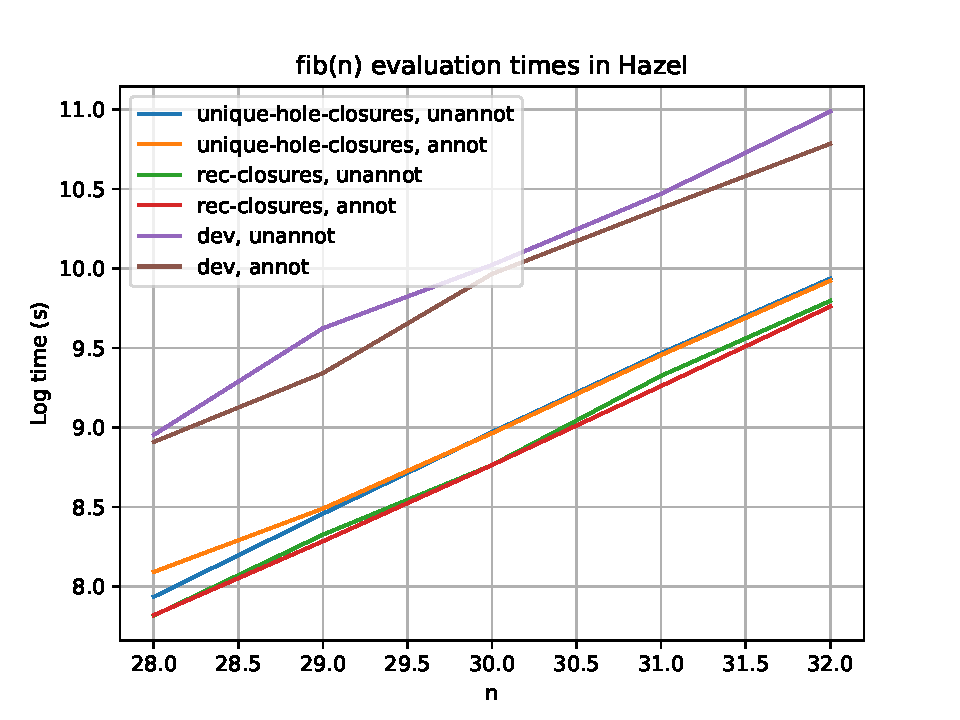
\includegraphics[width=10cm]{img/subst_evalenv_fib_perf.pdf}
%   \caption{Performance of the different models of evaluation}
%   \label{fig:perf_evaluation_models}
% \end{figure}

\begin{listing}
  \inputhminted{perf_fib}
  \caption{An evaluation-heavy Hazel program with no holes}
  \label{fig:perf-fib}
\end{listing}

\begin{singlespace}
  \begin{table}
    \centering
    \begin{tabular}{r|ccc}
      \hline
      $n$ & \texttt{dev} branch & \texttt{eval-environment} branch & \texttt{rec-closures} branch \\
      \hline\hline
      22 & 537 & 255 & 272 \\
      23 & 871 & 406 & 374 \\
      24 & 1270 & 578 & 552 \\
      25 & 1925 & 851 & 831 \\
      26 & 3048 & 1318 & 1297 \\
      \hline\hline
    \end{tabular}
    \caption{Time (ms) to compute $\text{fib}(n)$}
    \label{tab:perf-fib}
  \end{table}
\end{singlespace}

\todo{also compare the performance of the above with the recursive data structures example}

\begin{listing}
  \inputhminted{perf_fib_more_bindings}
  \caption{An evaluation-heavy Hazel program with more variable bindings}
  \label{fig:perf-fib-more-bindings}
\end{listing}

\begin{singlespace}
  \begin{table}
    \centering
    \begin{tabular}{r|cc}
      \hline
      $n$ & \texttt{dev} branch & \texttt{eval-environment} branch \\
      \hline\hline
      22 & 360 & 399 \\
      23 & 516 & 566 \\
      24 & 834 & 837 \\
      25 & 1257 & 1315 \\
      26 & 2090 & 2088 \\
      \hline\hline
    \end{tabular}
    \caption{Time (ms) to compute $\text{fib}(n)$ with more bound variables}
    \label{tab:perf-fib-more-bindings}
  \end{table}
\end{singlespace}

\todo{note that there is now a "prologue" of some builtin functions: PI, int\_of\_float, float\_of\_int, and mod; these cause lookups to be slower because they take part of each lookup operation}

\begin{listing}
  \inputhminted{perf_fib_more_branches}
  \caption{An evaluation-heavy Hazel program with unused variable substitutions}
  \label{fig:perf-fib-more-branches}
\end{listing}

\begin{singlespace}
  \begin{table}
    \centering
    \begin{tabular}{r|cc}
      \hline
      $n$ & \texttt{dev} branch & \texttt{eval-environment} branch \\
      \hline\hline
      22 & 495 & 377 \\
      23 & 772 & 551 \\
      24 & 1224 & 872 \\
      25 & 1977 & 1378 \\
      26 & 3149 & 2205 \\
      \hline\hline
    \end{tabular}
    \caption{Time (ms) to compute $\text{fib}(n)$ with substitutions in unused branches}
    \label{tab:perf-fib-more-branches}
  \end{table}
\end{singlespace}

\section{Postprocessing performance}
\label{sec:evaluation-renumbering}

Consider the set of programs described by \Cref{fig:hole_renumbering_problem}.

\todo{describe this code blowup example}

\begin{singlespace}
  \begin{table}
    \centering
    \begin{tabular}{r|ccc|ccc}
      \hline
      & \multicolumn{3}{c|}{\texttt{dev} branch} & \multicolumn{3}{c}{\texttt{eval-environment} branch} \\
      & Evaluate & Postprocessing & Equality & Evaluate & Postprocessing & Equality \\
      \hline\hline
      1 & 0 & 0 & 0 & 0 & 1 & 0 \\
      2 & 0 & 0 & 0 & 0 & 1 & 0 \\
      3 & 1 & 2 & 0 & 0 & 1 & 0 \\
      4 & 1 & 1 & 1 & 1 & 0 & 0 \\
      5 & 1 & 1 & 2 & 0 & 3 & 0 \\
      6 & 5 & 1 & 3 & 1 & 0 & 0 \\
      7 & 4 & 5 & 6 & 2 & 2 & 0 \\
      8 & 3 & 3 & 14 & 0 & 0 & 0 \\
      9 & 6 & 18 & 33 & 1 & 0 & 1 \\
      10 & 14 & 29 & 61 & 0 & 0 & 0 \\
      11 & 13 & 41 & 91 & 3 & 2 & 0 \\
      12 & 25 & 145 & 203 & 2 & 0 & 1 \\
      13 & 65 & 578 & 383 & 2 & 0 & 0 \\
      14 & 147 & 2399 & 924 & 1 & 3 & 1 \\
      15 & 226 & 16597 & 1603 & 3 & 0 & 1 \\
      16 & & & & 1 & 0 & 1 \\
      17 & & & & 2 & 1 & 1 \\
      18 & & & & 0 & 3 & 1 \\
      19 & & & & 0 & 0 & 1 \\
      20 & & & & 3 & 4 & 0 \\
      21 & & & & 2 & 0 & 1 \\
      22 & & & & 0 & 2 & 1 \\
      23 & & & & 0 & 3 & 1 \\
      24 & & & & 0 & 6 & 1 \\
      25 & & & & 1 & 4 & 1 \\
      26 & & & & 1 & 2 & 1 \\
      \hline\hline
    \end{tabular}
    \caption{Performance of program illustrated in \Cref{fig:hole_renumbering_problem}}
    \label{tab:perf-hole-blowup}
  \end{table}
\end{singlespace}

\section{FAR performance}
\label{sec:evaluation-far}

\begin{singlespace}
  \begin{table}
    \centering
    \begin{tabular}{p{10em}cccc}
      \hline
      Program & Steps & Steps & Step $\Delta$ & Cumulative \\
              & & (w/ FAR) & & Step $\Delta$ \\
      \hline\hline
      \inputhnfminted{far_fib_hist_1} & 7 & - & 0 & 0 \\ \hline
      \inputhnfminted{far_fib_hist_2} & 12 & 21 & 9 & 9 \\ \hline
      \inputhnfminted{far_fib_hist_3} & 17 & - & 0 & 9 \\ \hline
      \inputhnfminted{far_fib_hist_4} & 58 & 69 & 11 & 20 \\ \hline
      \inputhnfminted{far_fib_hist_5} & 4762964 & - & 0 & 20 \\ \hline
      \inputhnfminted{far_fib_hist_6} & 4762966 & 12 & -4762954 & -4762934 \\ \hline
      \inputhnfminted{far_fib_hist_7} & 4762966 & 21 & -4762954 & -9525879 \\ \hline
      \inputhnfminted{far_fib_hist_8} & 4792967 & 13 & -4792954 & -14288813 \\ \hline
      \hline
    \end{tabular}
    \caption{A program edit history with an expensive computation}
    \label{fig:far-program-history-fib}
  \end{table}
\end{singlespace}

\begin{singlespace}
  \begin{table}
    \centering
    \begin{tabular}{p{10em}cccc}
      \hline
      Program & Steps & Steps & Step $\Delta$ & Cumulative \\
              & & (w/ FAR) & & Step $\Delta$ \\
      \hline\hline
      \inputhnfminted{far_hist_1} & 1 & - & 0 & 0 \\ \hline
      \inputhnfminted{far_hist_2} & 2 & 3 & 1 & 1 \\ \hline
      \inputhnfminted{far_hist_3} & 3 & - & 0 & 1 \\ \hline
      \inputhnfminted{far_hist_4} & 4 & 5 & 1 & 2 \\ \hline
      \inputhnfminted{far_hist_5} & 5 & - & 0 & 2 \\ \hline
      \inputhnfminted{far_hist_6} & 6 & 9 & 3 & 5 \\ \hline
      \inputhnfminted{far_hist_7} & 8 & 8 & 0 & 5 \\ \hline
      \inputhnfminted{far_hist_8} & 9 & 14 & 5 & 10 \\ \hline
      \inputhnfminted{far_hist_9} & 10 & 11 & 1 & 11 \\ \hline
      \inputhnfminted{far_hist_10} & 11 & 6 & -5 & 6 \\ \hline
      \hline
    \end{tabular}
    \caption{A sample edit history for a simple program}
    \label{fig:far-program-history-simple}
  \end{table}
\end{singlespace}

%%% Local Variables:
%%% mode: latex
%%% TeX-master: "main"
%%% End:
